
%% bare_conf_compsoc.tex
%% V1.4b
%% 2015/08/26
%% by Michael Shell
%% See:
%% http://www.michaelshell.org/
%% for current contact information.
%%
%% This is a skeleton file demonstrating the use of IEEEtran.cls
%% (requires IEEEtran.cls version 1.8b or later) with an IEEE Computer
%% Society conference paper.
%%
%% Support sites:
%% http://www.michaelshell.org/tex/ieeetran/
%% http://www.ctan.org/pkg/ieeetran
%% and
%% http://www.ieee.org/

%%*************************************************************************
%% Legal Notice:
%% This code is offered as-is without any warranty either expressed or
%% implied; without even the implied warranty of MERCHANTABILITY or
%% FITNESS FOR A PARTICULAR PURPOSE! 
%% User assumes all risk.
%% In no event shall the IEEE or any contributor to this code be liable for
%% any damages or losses, including, but not limited to, incidental,
%% consequential, or any other damages, resulting from the use or misuse
%% of any information contained here.
%%
%% All comments are the opinions of their respective authors and are not
%% necessarily endorsed by the IEEE.
%%
%% This work is distributed under the LaTeX Project Public License (LPPL)
%% ( http://www.latex-project.org/ ) version 1.3, and may be freely used,
%% distributed and modified. A copy of the LPPL, version 1.3, is included
%% in the base LaTeX documentation of all distributions of LaTeX released
%% 2003/12/01 or later.
%% Retain all contribution notices and credits.
%% ** Modified files should be clearly indicated as such, including  **
%% ** renaming them and changing author support contact information. **
%%*************************************************************************


% *** Authors should verify (and, if needed, correct) their LaTeX system  ***
% *** with the testflow diagnostic prior to trusting their LaTeX platform ***
% *** with production work. The IEEE's font choices and paper sizes can   ***
% *** trigger bugs that do not appear when using other class files.       ***                          ***
% The testflow support page is at:
% http://www.michaelshell.org/tex/testflow/



\documentclass[conference,compsoc]{IEEEtran}
\usepackage{graphicx}
\usepackage{listings}

% Some/most Computer Society conferences require the compsoc mode option,
% but others may want the standard conference format.
%
% If IEEEtran.cls has not been installed into the LaTeX system files,
% manually specify the path to it like:
% \documentclass[conference,compsoc]{../sty/IEEEtran}





% Some very useful LaTeX packages include:
% (uncomment the ones you want to load)


% *** MISC UTILITY PACKAGES ***
%
%\usepackage{ifpdf}
% Heiko Oberdiek's ifpdf.sty is very useful if you need conditional
% compilation based on whether the output is pdf or dvi.
% usage:
% \ifpdf
%   % pdf code
% \else
%   % dvi code
% \fi
% The latest version of ifpdf.sty can be obtained from:
% http://www.ctan.org/pkg/ifpdf
% Also, note that IEEEtran.cls V1.7 and later provides a builtin
% \ifCLASSINFOpdf conditional that works the same way.
% When switching from latex to pdflatex and vice-versa, the compiler may
% have to be run twice to clear warning/error messages.






% *** CITATION PACKAGES ***
%
\ifCLASSOPTIONcompsoc
  % IEEE Computer Society needs nocompress option
  % requires cite.sty v4.0 or later (November 2003)
  \usepackage[nocompress]{cite}
\else
  % normal IEEE
  \usepackage{cite}
\fi
% cite.sty was written by Donald Arseneau
% V1.6 and later of IEEEtran pre-defines the format of the cite.sty package
% \cite{} output to follow that of the IEEE. Loading the cite package will
% result in citation numbers being automatically sorted and properly
% "compressed/ranged". e.g., [1], [9], [2], [7], [5], [6] without using
% cite.sty will become [1], [2], [5]--[7], [9] using cite.sty. cite.sty's
% \cite will automatically add leading space, if needed. Use cite.sty's
% noadjust option (cite.sty V3.8 and later) if you want to turn this off
% such as if a citation ever needs to be enclosed in parenthesis.
% cite.sty is already installed on most LaTeX systems. Be sure and use
% version 5.0 (2009-03-20) and later if using hyperref.sty.
% The latest version can be obtained at:
% http://www.ctan.org/pkg/cite
% The documentation is contained in the cite.sty file itself.
%
% Note that some packages require special options to format as the Computer
% Society requires. In particular, Computer Society  papers do not use
% compressed citation ranges as is done in typical IEEE papers
% (e.g., [1]-[4]). Instead, they list every citation separately in order
% (e.g., [1], [2], [3], [4]). To get the latter we need to load the cite
% package with the nocompress option which is supported by cite.sty v4.0
% and later.





% *** GRAPHICS RELATED PACKAGES ***
%
\ifCLASSINFOpdf
  % \usepackage[pdftex]{graphicx}
  % declare the path(s) where your graphic files are
  % \graphicspath{{../pdf/}{../jpeg/}}
  % and their extensions so you won't have to specify these with
  % every instance of \includegraphics
  % \DeclareGraphicsExtensions{.pdf,.jpeg,.png}
\else
  % or other class option (dvipsone, dvipdf, if not using dvips). graphicx
  % will default to the driver specified in the system graphics.cfg if no
  % driver is specified.
  % \usepackage[dvips]{graphicx}
  % declare the path(s) where your graphic files are
  % \graphicspath{{../eps/}}
  % and their extensions so you won't have to specify these with
  % every instance of \includegraphics
  % \DeclareGraphicsExtensions{.eps}
\fi
% graphicx was written by David Carlisle and Sebastian Rahtz. It is
% required if you want graphics, photos, etc. graphicx.sty is already
% installed on most LaTeX systems. The latest version and documentation
% can be obtained at: 
% http://www.ctan.org/pkg/graphicx
% Another good source of documentation is "Using Imported Graphics in
% LaTeX2e" by Keith Reckdahl which can be found at:
% http://www.ctan.org/pkg/epslatex
%
% latex, and pdflatex in dvi mode, support graphics in encapsulated
% postscript (.eps) format. pdflatex in pdf mode supports graphics
% in .pdf, .jpeg, .png and .mps (metapost) formats. Users should ensure
% that all non-photo figures use a vector format (.eps, .pdf, .mps) and
% not a bitmapped formats (.jpeg, .png). The IEEE frowns on bitmapped formats
% which can result in "jaggedy"/blurry rendering of lines and letters as
% well as large increases in file sizes.
%
% You can find documentation about the pdfTeX application at:
% http://www.tug.org/applications/pdftex





% *** MATH PACKAGES ***
%
%\usepackage{amsmath}
% A popular package from the American Mathematical Society that provides
% many useful and powerful commands for dealing with mathematics.
%
% Note that the amsmath package sets \interdisplaylinepenalty to 10000
% thus preventing page breaks from occurring within multiline equations. Use:
%\interdisplaylinepenalty=2500
% after loading amsmath to restore such page breaks as IEEEtran.cls normally
% does. amsmath.sty is already installed on most LaTeX systems. The latest
% version and documentation can be obtained at:
% http://www.ctan.org/pkg/amsmath





% *** SPECIALIZED LIST PACKAGES ***
%
%\usepackage{algorithmic}
% algorithmic.sty was written by Peter Williams and Rogerio Brito.
% This package provides an algorithmic environment fo describing algorithms.
% You can use the algorithmic environment in-text or within a figure
% environment to provide for a floating algorithm. Do NOT use the algorithm
% floating environment provided by algorithm.sty (by the same authors) or
% algorithm2e.sty (by Christophe Fiorio) as the IEEE does not use dedicated
% algorithm float types and packages that provide these will not provide
% correct IEEE style captions. The latest version and documentation of
% algorithmic.sty can be obtained at:
% http://www.ctan.org/pkg/algorithms
% Also of interest may be the (relatively newer and more customizable)
% algorithmicx.sty package by Szasz Janos:
% http://www.ctan.org/pkg/algorithmicx




% *** ALIGNMENT PACKAGES ***
%
%\usepackage{array}
% Frank Mittelbach's and David Carlisle's array.sty patches and improves
% the standard LaTeX2e array and tabular environments to provide better
% appearance and additional user controls. As the default LaTeX2e table
% generation code is lacking to the point of almost being broken with
% respect to the quality of the end results, all users are strongly
% advised to use an enhanced (at the very least that provided by array.sty)
% set of table tools. array.sty is already installed on most systems. The
% latest version and documentation can be obtained at:
% http://www.ctan.org/pkg/array


% IEEEtran contains the IEEEeqnarray family of commands that can be used to
% generate multiline equations as well as matrices, tables, etc., of high
% quality.




% *** SUBFIGURE PACKAGES ***
%\ifCLASSOPTIONcompsoc
%  \usepackage[caption=false,font=footnotesize,labelfont=sf,textfont=sf]{subfig}
%\else
%  \usepackage[caption=false,font=footnotesize]{subfig}
%\fi
% subfig.sty, written by Steven Douglas Cochran, is the modern replacement
% for subfigure.sty, the latter of which is no longer maintained and is
% incompatible with some LaTeX packages including fixltx2e. However,
% subfig.sty requires and automatically loads Axel Sommerfeldt's caption.sty
% which will override IEEEtran.cls' handling of captions and this will result
% in non-IEEE style figure/table captions. To prevent this problem, be sure
% and invoke subfig.sty's "caption=false" package option (available since
% subfig.sty version 1.3, 2005/06/28) as this is will preserve IEEEtran.cls
% handling of captions.
% Note that the Computer Society format requires a sans serif font rather
% than the serif font used in traditional IEEE formatting and thus the need
% to invoke different subfig.sty package options depending on whether
% compsoc mode has been enabled.
%
% The latest version and documentation of subfig.sty can be obtained at:
% http://www.ctan.org/pkg/subfig




% *** FLOAT PACKAGES ***
%
%\usepackage{fixltx2e}
% fixltx2e, the successor to the earlier fix2col.sty, was written by
% Frank Mittelbach and David Carlisle. This package corrects a few problems
% in the LaTeX2e kernel, the most notable of which is that in current
% LaTeX2e releases, the ordering of single and double column floats is not
% guaranteed to be preserved. Thus, an unpatched LaTeX2e can allow a
% single column figure to be placed prior to an earlier double column
% figure.
% Be aware that LaTeX2e kernels dated 2015 and later have fixltx2e.sty's
% corrections already built into the system in which case a warning will
% be issued if an attempt is made to load fixltx2e.sty as it is no longer
% needed.
% The latest version and documentation can be found at:
% http://www.ctan.org/pkg/fixltx2e


%\usepackage{stfloats}
% stfloats.sty was written by Sigitas Tolusis. This package gives LaTeX2e
% the ability to do double column floats at the bottom of the page as well
% as the top. (e.g., "\begin{figure*}[!b]" is not normally possible in
% LaTeX2e). It also provides a command:
%\fnbelowfloat
% to enable the placement of footnotes below bottom floats (the standard
% LaTeX2e kernel puts them above bottom floats). This is an invasive package
% which rewrites many portions of the LaTeX2e float routines. It may not work
% with other packages that modify the LaTeX2e float routines. The latest
% version and documentation can be obtained at:
% http://www.ctan.org/pkg/stfloats
% Do not use the stfloats baselinefloat ability as the IEEE does not allow
% \baselineskip to stretch. Authors submitting work to the IEEE should note
% that the IEEE rarely uses double column equations and that authors should try
% to avoid such use. Do not be tempted to use the cuted.sty or midfloat.sty
% packages (also by Sigitas Tolusis) as the IEEE does not format its papers in
% such ways.
% Do not attempt to use stfloats with fixltx2e as they are incompatible.
% Instead, use Morten Hogholm'a dblfloatfix which combines the features
% of both fixltx2e and stfloats:
%
% \usepackage{dblfloatfix}
% The latest version can be found at:
% http://www.ctan.org/pkg/dblfloatfix




% *** PDF, URL AND HYPERLINK PACKAGES ***
%
%\usepackage{url}
% url.sty was written by Donald Arseneau. It provides better support for
% handling and breaking URLs. url.sty is already installed on most LaTeX
% systems. The latest version and documentation can be obtained at:
% http://www.ctan.org/pkg/url
% Basically, \url{my_url_here}.




% *** Do not adjust lengths that control margins, column widths, etc. ***
% *** Do not use packages that alter fonts (such as pslatex).         ***
% There should be no need to do such things with IEEEtran.cls V1.6 and later.
% (Unless specifically asked to do so by the journal or conference you plan
% to submit to, of course. )


% correct bad hyphenation here
\hyphenation{op-tical net-works semi-conduc-tor}


\begin{document}
%
% paper title
% Titles are generally capitalized except for words such as a, an, and, as,
% at, but, by, for, in, nor, of, on, or, the, to and up, which are usually
% not capitalized unless they are the first or last word of the title.
% Linebreaks \\ can be used within to get better formatting as desired.
% Do not put math or special symbols in the title.
\title{Intelligent Monitoring and Risk Assessment \\for Gestational Diabetes Mellitus (GDM)}


% author names and affiliations
% use a multiple column layout for up to three different
% affiliations
\author{\IEEEauthorblockN{Shwetha Saravanan}
\IEEEauthorblockA{School of Electrical and\\Computer Engineering\\
University of Waterloo\\
Waterloo ID: 21005381}
\and
\IEEEauthorblockN{Ope Salau}
\IEEEauthorblockA{School of Electrical and\\Computer Engineering\\
University of Waterloo\\
Waterloo ID:20435961}
\and
\IEEEauthorblockN{Saurav Bin Saji}
\IEEEauthorblockA{School of Electrical and\\Computer Engineering\\
University of Waterloo\\
Waterloo ID: 21041330\\
}
}


% conference papers do not typically use \thanks and this command
% is locked out in conference mode. If really needed, such as for
% the acknowledgment of grants, issue a \IEEEoverridecommandlockouts
% after \documentclass

% for over three affiliations, or if they all won't fit within the width
% of the page (and note that there is less available width in this regard for
% compsoc conferences compared to traditional conferences), use this
% alternative format:
% 
%\author{\IEEEauthorblockN{Michael Shell\IEEEauthorrefmark{1},
%Homer Simpson\IEEEauthorrefmark{2},
%James Kirk\IEEEauthorrefmark{3}, 
%Montgomery Scott\IEEEauthorrefmark{3} and
%Eldon Tyrell\IEEEauthorrefmark{4}}
%\IEEEauthorblockA{\IEEEauthorrefmark{1}School of Electrical and Computer Engineering\\
%Georgia Institute of Technology,
%Atlanta, Georgia 30332--0250\\ Email: see http://www.michaelshell.org/contact.html}
%\IEEEauthorblockA{\IEEEauthorrefmark{2}Twentieth Century Fox, Springfield, USA\\
%Email: homer@thesimpsons.com}
%\IEEEauthorblockA{\IEEEauthorrefmark{3}Starfleet Academy, San Francisco, California 96678-2391\\
%Telephone: (800) 555--1212, Fax: (888) 555--1212}
%\IEEEauthorblockA{\IEEEauthorrefmark{4}Tyrell Inc., 123 Replicant Street, Los Angeles, California 90210--4321}}




% use for special paper notices
%\IEEEspecialpapernotice{(Invited Paper)}




% make the title area
\maketitle

% As a general rule, do not put math, special symbols or citations
% in the abstract
\begin{abstract}
High blood glucose levels brought on by hormonal changes that lessen insulin effectiveness are symptoms of gestational diabetes mellitus (GDM), which is dangerous for both pregnant women and their unborn children. Despite the fact that most GDM symptoms go away after delivery, newborns still run the risk of hypoglycemia and macrosomia. It is essential to closely monitor the mother's blood sugar levels when she is in labour. Real-time monitoring utilising biosensors to gather information on blood pressure, BMI, and glucose levels is one of the solutions that has been suggested. Simulated data has been used due to hardware limitations. Access control and encryption would be used to store the data in a secure cloud infrastructure. Using machine learning and deep learning models trained on online datasets, risk analysis would be carried out. Applications for users and providers would help with communication and alert medical staff. Implementing this plan improves maternal and fetal health by fostering coordinated care, risk assessment, and proactive management for pregnant women with GDM. Real-time data collection from pregnant women presents difficulties that can be overcome by trained algorithms and simulated data.
\end{abstract}

% no keywords


% For peer review papers, you can put extra information on the cover
% page as needed:
% \ifCLASSOPTIONpeerreview
% \begin{center} \bfseries EDICS Category: 3-BBND \end{center}
% \fi
%
% For peerreview papers, this IEEEtran command inserts a page break and
% creates the second title. It will be ignored for other modes.
\IEEEpeerreviewmaketitle



\section{Introduction}
Gestational Diabetes Mellitus (GDM) is a significant health concern affecting pregnant women worldwide. It is characterized by high blood glucose levels during pregnancy, primarily caused by hormonal changes that reduce insulin effectiveness and promote insulin resistance. GDM poses serious risks not only to the expectant mother but also to the health and well-being of the unborn child. Although most GDM symptoms tend to resolve after delivery, the newborns still face potential complications, such as hypoglycemia (low blood sugar) and macrosomia (excessive fetal growth).During pregnancy, the placenta produces hormones that can interfere with the proper utilization of insulin in the mother's body, leading to elevated blood sugar levels. These high blood glucose levels can have detrimental effects on both maternal health and fetal development. Pregnant women with GDM are at an increased risk of experiencing complications, including preeclampsia, cesarean deliveries, and the need for labor induction. Moreover, the newborns are susceptible to issues arising from the abrupt change in glucose levels after birth, putting them at risk of hypoglycemia and macrosomia.

The newborn may continue to have issues with elevated blood glucose levels after birth. The body of the newborn has adjusted to the greater glucose levels in the mother's circulation, so when they are separated, the quick reduction in glucose might cause hypoglycemia. Newborns with hypoglycemia may have a dangerous condition that needs quick medical intervention. A typical side effect of GDM is macrosomia or excessive fetal growth. The baby's pancreas may create more insulin as a result of the mother's blood glucose levels being elevated, which could speed up the baby's growth. Babies with macrosomia are more likely to have birth trauma, such as shoulder dystocia (difficulty delivering the shoulders), and may also require an assisted delivery or cesarean section.

The mother's blood glucose levels must be closely monitored throughout labor to reduce the hazards related to GDM. This monitoring enables medical practitioners to keep the mother's blood sugar levels regular, which helps to avoid complications for the newborn after birth. For blood glucose control during labor, insulin or other drugs may occasionally be used.

Gestational diabetes mellitus (GDM) is the need of the hour due to several reasons:
\begin{itemize}
    \item Implications for Maternal Health: GDM can have detrimental implications on a woman's health while she is expecting, including a higher chance of type 2 diabetes in the future. We can lessen these long-term health concerns for women by tackling GDM.

   \item Risks to the fetus and newborn: Children born to moms with GDM run the risk of developing problems like hypoglycemia and macrosomia. Early detection and treatment of GDM during labor can lower these risks and enhance neonatal outcomes.
\item Opportunities for Early Intervention: GDM offers a chance for early detection and intervention in the management of diabetes. Healthcare practitioners can effectively manage GDM by implementing suitable interventions and lifestyle changes by constantly monitoring blood glucose levels throughout pregnancy.

\item Long-term Health Impact: GDM has effects on mothers' and babies' long-term health in addition to their immediate health. Effective GDM management can lower long- and short-term risks of acquiring diabetes and its consequences.

\item Holistic Maternal and Foetal Care: Treating GDM is crucial to offering pregnant women and their unborn children all-encompassing, holistic care. Healthcare providers can customize treatment plans and actions to address the particular needs of each patient by putting into place efficient monitoring and risk assessment strategies.
\end{itemize}
Infants of mothers with gestational diabetes mellitus (GDM) are more likely to experience macrosomia, which is excessive foetal growth that causes a higher birth weight. Maternal BMI, insulin resistance, foetal biometric measures, and glucose levels are some of the factors that go into determining the risk of macrosomia. Low blood sugar in infants is known as hypoglycemia and develops after birth as a result of the abrupt reduction in the supply of glucose. Maternal glucose management, the timing of delivery, newborn blood glucose levels, and signs and symptoms are all factors in determining hypoglycemia risk.

To address the increasing prevalence of gestational diabetes mellitus (GDM), routine screening during prenatal care is crucial. However, universal testing for GDM is not uniformly implemented worldwide. In the United States, the American College of Obstetricians and Gynecologists (ACOG) recommends all pregnant women to undergo testing between 24 and 28 weeks of gestation. In other countries, screening is based on individual risk assessments conducted by obstetricians. Risk categories include low, average, and very high, taking into account factors such as age, pre-pregnancy weight, ethnicity, family history of diabetes, and obstetric history.

This project implements a comprehensive solution for healthcare professionals to effectively monitor glucose levels, evaluate risks, and take proactive steps to address the challenges faced by expectant women with GDM. The project aims to enhance coordinated care, improve maternal and fetal well-being, and promote the integration of clinical guidelines and best practices into the decision support system.

\subsection{Literature Survey}
  Gestational Diabetes Mellitus (GDM) monitoring System,  an innovative and much-needed solution that aims to revolutionize the care provided to pregnant women with GDM. With its novel approach and advanced features, this project addresses the critical need for efficient monitoring, accurate risk assessment, and seamless communication among healthcare professionals, pregnant women, and stakeholders. By leveraging state-of-the-art technologies such as real-time data collection, secure cloud processing, and machine learning integration, our project fills a crucial gap in the current healthcare landscape. With its impact potential, the GDM Management System promises to transform the management of GDM, ensuring the optimal health and well-being of both mothers and babies throughout the pregnancy journey.

The authors of Kurt et al.'s study [1] suggest a prediction model for GDM that makes use of deep learning and Bayesian optimization methods. The study emphasizes the value of using cutting-edge machine learning methods to forecast GDM. The authors achieve great accuracy in GDM prediction by utilizing a sizable dataset and optimizing the model parameters using Bayesian optimization.
Two important studies that are re are examined in the literature review that follows: [1] and [2]. The findings support the objective of our study, which is to use machine learning integration for risk analysis, by demonstrating the capability of deep learning algorithms to efficiently analyze sequential data, such as patient clinical data.

El-Rashidy et al. [2] address the prediction of GDM based on explainable deep learning and fog computing in another pertinent study. The authors place a strong emphasis on the use of interpretable models for aiding in decision-making and offering insights into the prediction process. In order to improve prediction efficiency and accuracy, the study offers a unique fog computing system that integrates local and cloud-based resources. Healthcare practitioners can build targeted interventions by using explainable deep learning techniques to help them comprehend the fundamental causes of GDM prediction. This is in line with our project's objective, which is to build a risk analysis system that gives healthcare providers transparent risk evaluations and clear explanations.

The promise of advanced machine learning and deep learning techniques to forecast GDM, enhance risk assessment capabilities, and guide clinical decision-making is highlighted in both articles. Accurate and trustworthy GDM prediction is made possible by the use of huge datasets, optimization techniques, and the incorporation of interpretability. These results lend credence to the justification for our project's strategy of integrating machine learning and deep learning for risk assessments while utilizing trained models from internet sources.
The literature study emphasizes the significance of utilizing cutting-edge deep learning and machine learning approaches for precise risk assessment and prediction in GDM management. The works by Kurt et al. [1] and El-Rashidy et al. [2] offer insightful techniques that are consistent with the goals of our endeavor. We improve the decision support system and risk analysis capabilities in our project by incorporating these data, which will ultimately improve the management and outcomes of GDM.

\subsection{Proposed Architecture}

We propose to perform OGTT at home where a standard glucometer is used  to perform the Oral Glucose Tolerance Test (OGTT).This modified approach to perform the OGTT at home using a standard glucometer equipped with Bluetooth technology. The modified glucometer will allow seamless connectivity to the user's device and transmit the data via WiFi to the cloud for further analysis. Additionally, the collected data will be visualized in real-time through a user-friendly web application. 


\section{Experimental Setup}
\subsection{Hardware Design System}
\subsubsection{Conventional Methodology}\\

A diagnostic examination called the Oral Glucose Tolerance examination (OGTT) measures how well the body metabolizes glucose. GDM is frequently diagnosed using this method. The patient drinks a beverage during an OGTT that normally contains 75 g of glucose. After that, blood glucose levels are monitored at predetermined intervals to gauge how the body is handling the glucose load.

A fasting blood sample is taken before ingesting the glucose beverage as the first step in the OGTT, which normally entails repeated blood glucose readings. At regular intervals, such as an hour and two hours after ingesting the glucose solution, further blood samples are obtained. These blood samples aid in assessing how well the body eliminates glucose from the bloodstream and processes it.

Age, BMI, OGTT, and ethnicity are the main influencing factors that predict gestational diabetes mellitus (GDM), according to considerable literature and consultations with obstetricians. Due to lifestyle variables and other characteristics, Asian populations tend to have a higher incidence of these criteria, which have been found to be significant predictors of the development of GDM.

\subsubsection{Glucometer Functioning }

On the basis of electrochemical measurement principles, the traditional glucose metre functions. In order to interact with a blood sample, electrochemical blood glucose test strips (EBGTS) use an enzymatic process involving mediators and glucose oxidase. Using calibration curves and algorithms, the resulting electric current is measured and transformed into glucose concentration. Conventional glucometers are extensively used, however they have drawbacks in terms of calibration errors, response times, and data accessibility.
The electrochemical technology used to measure the glucose concentration in a blood sample is the basis for a glucometer's operation. The electronic equipment and test strips are combined to turn the glucose level into a measurable voltage. Here is a thorough description of how a glucometer functions and how it converts the glucose level into voltage to display the glucose level is explained below:
\begin{enumerate}
    
    \item Application of Test Strip and Sample:
The user begins by applying a little amount of blood (often obtained by puncturing the fingertip) onto a temporary test strip. Electrodes, enzymes, and mediators are only a few of the parts that make up the test strip.
    \item Biological Reaction:
The test strip contains an enzyme (often glucose oxidase) that reacts with the glucose in the blood sample. Byproducts of this enzymatic reaction include hydrogen peroxide (H2O2) and the conversion of the glucose molecule.

\item Convert to Voltage:
An electrical current is produced in the test strip as a result of the transport of electrons to the mediator.The amount of this current is inversely correlated with the blood sample's glucose concentration. In other words, electrical currents increase when glucose levels rise. An inverting amplifier is then used to increase the voltage that the current-to-voltage converter has converted. The micro-controller of the glucometer can continue processing the output after the amplifier has increased the voltage signal.

\item Processing by micro-controllers: The microcontroller of the glucometer receives the enhanced voltage. The inbuilt Analog-to-Digital Converter (ADC) of the micro-controller digitises the amplified voltage signal.

\item Calibration and algorithm: A conversion from the digitised voltage signal to the real blood glucose level is required. Calibration curves and algorithms kept in the microcontroller's memory are used to do this. The calibration curves are created from the relationship between the electrical current generated in the test strip and the associated glucose concentration during calibration using known glucose solutions.

\item Showing Blood Glucose Level: The glucose concentration in the blood sample is calculated by the microcontroller after it has processed the digitised voltage signal using the calibration curves and algorithms. Depending on the user's selection, the outcome is then shown on the glucometer's screen as the glucose level in either millimoles per litre (mmol/L) or milligrammes per deciliter (mg/dL), as appropriate.

\item Data Storage and Shut-Off: Glucometers automatically turn off after displaying the result in order to save battery. Many contemporary glucometers also include memory features, which enable devices to save multiple readings for later study or reference.
\end{enumerate}
A glucometer uses electrochemical processes to determine the amount of glucose present in a blood sample. The microprocessor processes the resulting electrical current to create a quantifiable voltage, which is then used to display the glucose level on the device's screen. This makes it simple for diabetics to check their blood glucose levels and properly control their condition.\\
\begin{figure}[htbp]
  \centering
  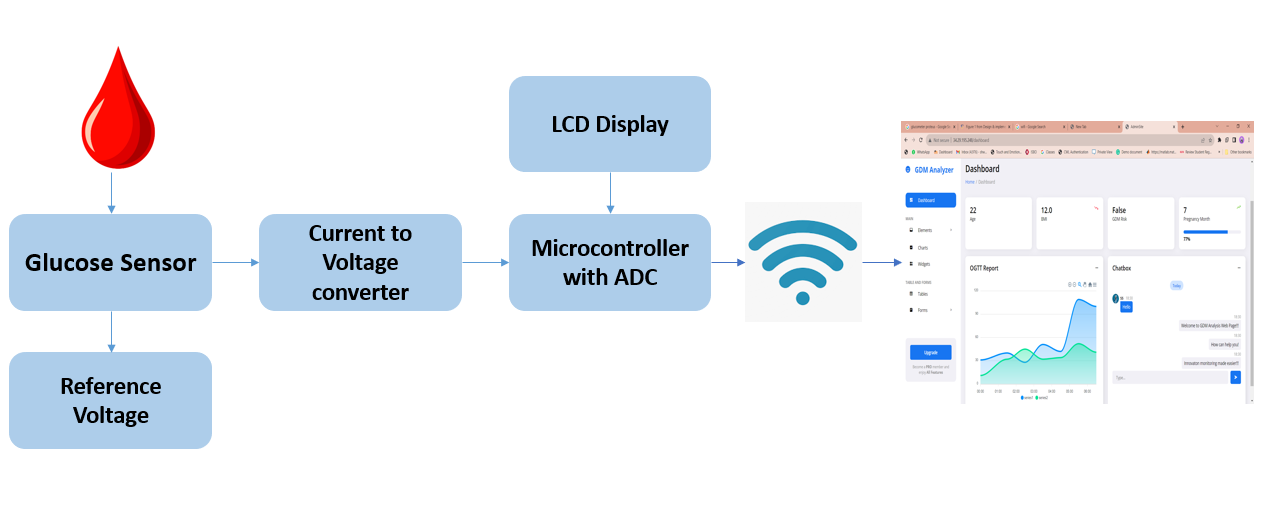
\includegraphics[width=0.8\columnwidth]{IEEEtran/glucometer_diag.PNG} % Replace with the actual path and filename of your image
  \caption{Proposed Functional flow of glucometer}
  \label{fig:glucometer_diag}
\end{figure}
The proposed glucometer integrates WiFi technology to address the limitations of conventional devices. The WiFi interface enables seamless connectivity with smartphones or other devices, allowing real-time transmission of glucose readings to a centralized database or cloud platform. This data can be remotely accessed by healthcare providers, facilitating timely interventions and personalized management for pregnant women with GDM.The hardware design incorporates an ESP8266 WiFi module with the glucometer's microcontroller, enabling wireless data transmission. Additionally, the system is equipped with a user-friendly interface for data visualization and glucose level trends, enhancing patient engagement and adherence to glucose monitoring protocols as shown in the Figure \ref{fig:glucometer_diag}..

\subsubsection{Data Acquisition}

The data-gathering procedure would involve the following steps to obtain the necessary information for risk assessment and monitoring:

Simulated OGTT readings: Due to hardware constraints, the sensor data from the glucometer is simulated using Python scripts. These scripts  generated simulated OGTT readings, including fasting glucose levels and glucose measurements at specified time intervals during the test.

User input for additional features: Users would be prompted to provide additional relevant information such as age, BMI, and ethnicity through the web application. Users would enter these details on the website, ensuring the availability of essential data for risk assessment and analysis.

By combining the simulated OGTT readings with the user-provided information, the ML/DL integration system can analyze the data and assess the risk of GDM based on the identified parameters. The simulated data allows for the evaluation of risk without requiring real-time measurements, while user input ensures the consideration of other significant factors.

This approach allows for efficient risk assessment and monitoring by leveraging simulated data and user-provided information. It enables healthcare professionals to identify high-risk cases, personalize treatment plans, and provide timely interventions for pregnant women with GDM. By considering parameters such as simulated OGTT readings, age, BMI, and ethnicity, this approach facilitates accurate risk assessment and targeted management of GDM throughout pregnancy.


\subsection{Predictor Model Analysis}

This study involves a predictive analysis to determine the presence of Gestational Diabetes Mellitus (GDM) in patients. The dataset consists of information from 26,063 patients and was collected from Figshare [4], a research data repository. Various factors such as Postcode, height, weight, BMI at booking, ethnicity, parity, results of glucose tolerance tests, mode of delivery, gestational age, neonatal birthweight, and other relevant features were considered. Data preprocessing, feature extraction, and encoding were performed to prepare the data for classification. Different machine learning classifiers were evaluated, and the Support Vector Classifier (SVC) showed the best performance.

\begin{figure}[!htbp]
  \centering
  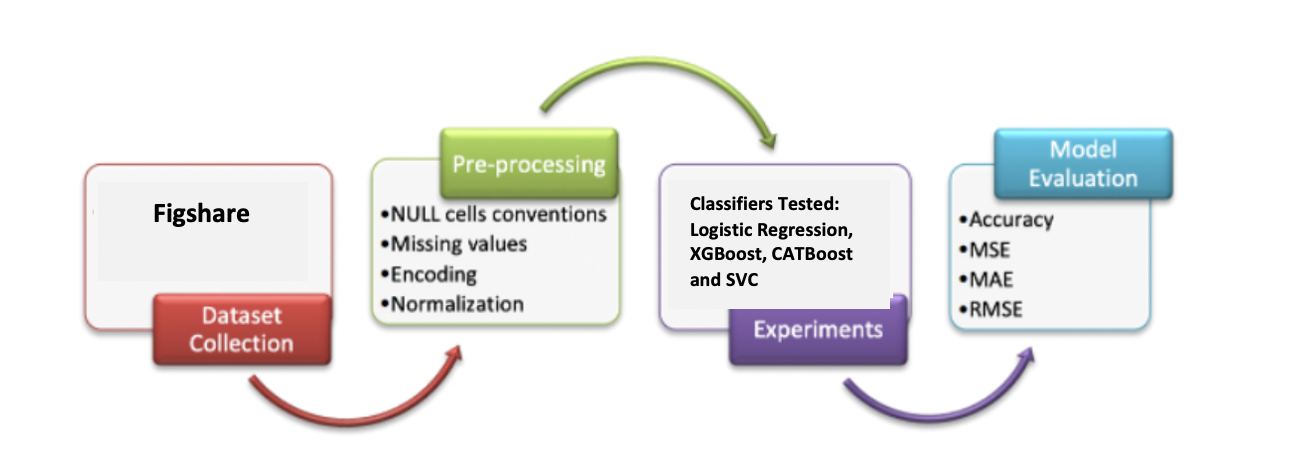
\includegraphics[width=0.8\columnwidth]{IEEEtran/Classifier_workflow.png} % Replace with the actual path and filename of your image
  \caption{Methodology of the Machine Learning Classifier}
  \label{fig:glucometer_diag}
\end{figure}

\subsubsection{Data Collection}
The dataset was obtained from Figshare and contains information on 26,063 patients. It includes various attributes related to pregnancy and health, such as demographics, glucose tolerance test results, and mode of delivery.

\subsubsection{Data Pre-processing}
To ensure data quality and consistency, we conducted data preprocessing. This involved handling missing values through null cell conversions and imputation. Categorical variables were encoded into numerical representations, and numerical features were normalized to bring them to a common scale.\\

\begin{itemize}

    \item \textbf{Null Cell Conversions}: In the dataset collected from Figshare, there may be instances where certain observations or attributes have missing values, referred to as null cells. To handle these missing values appropriately, an imputation approach was adopted rather than removing entire rows or columns with missing values. Various imputation methods were used, such as filling the missing values with the mean or median for numerical features like height, weight, and BMI at booking. For categorical features like ethnicity and mode of delivery, the mode (most frequent category) was used for imputation.\\

    \item \textbf{Filling Missing Values}: Filling missing values was an essential step in the data preprocessing phase. Specific imputation techniques were employed to replace the missing data with estimated values. For numerical features such as height, weight, and BMI at booking, missing values were filled by calculating the mean or median of the available data. For categorical features like ethnicity and mode of delivery, missing values were filled with the mode, representing the most frequent category for those features. In certain cases, machine learning models may have been used to predict missing values based on other relevant features.\\

    \item \textbf{Encoding}: Since machine learning classifiers require numerical inputs, categorical variables were converted into numerical representations using encoding techniques. For the GDM project, one-hot encoding was applied to handle categorical features such as ethnicity, parity, and mode of delivery. In one-hot encoding, each category within a categorical feature is transformed into a binary vector, where a '1' indicates the presence of that category, and '0' represents the absence. This encoding technique allowed the representation of categorical data in a way that could be effectively used by the machine learning models.\\

    \item \textbf{Normalization}: To ensure that numerical features with different scales do not dominate the training process, normalization was applied to bring them within a similar range. In the GDM project, the Min-Max scaling normalization technique was used for features such as height, weight, BMI, OGTT1h, and OGTT2h. This process scaled these features to a specific range, typically between 0 and 1, preserving the relative relationships between the data points while avoiding the influence of any feature's scale. Normalization ensured that all numerical features contributed equally to the model's performance during training and prediction. Additionally, it helped prevent any bias introduced by features with larger scales impacting the model's decision-making process.

\end{itemize}

\subsubsection{Feature Extraction and Encoding:}
To identify the most relevant features for predicting GDM, we performed feature extraction and correlation analysis. Features such as OGTT1h and OGTT2h exhibited the highest correlation with the target feature, GDM. Less relevant features were removed, resulting in a smaller dataset with the most significant features.

\subsubsection{Model Evaluation:}

\begin{figure}[!htbp]
  \centering
  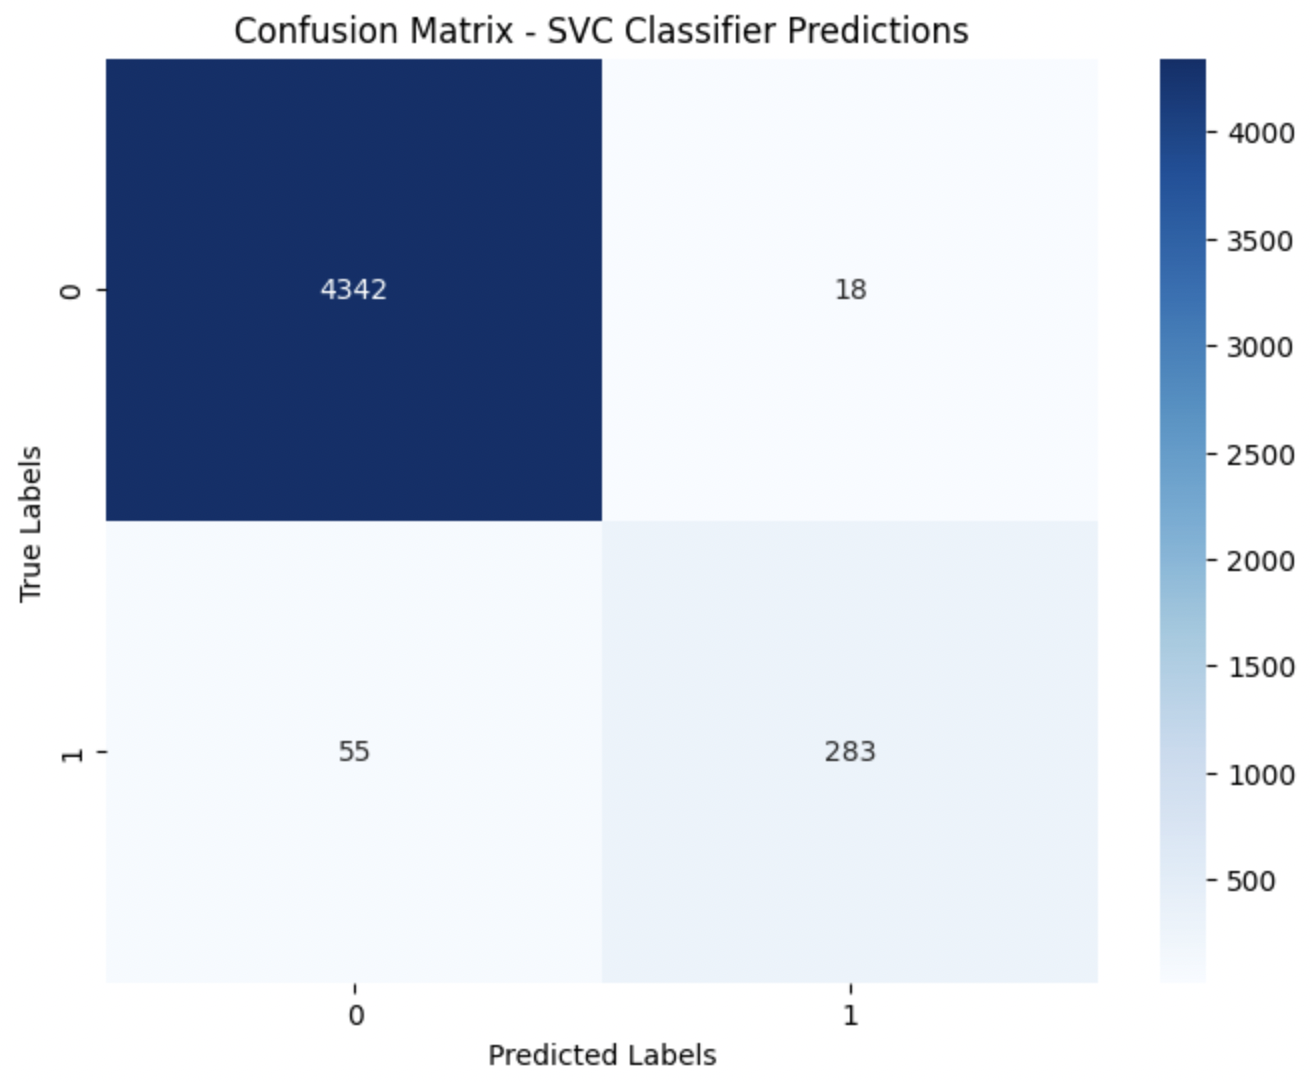
\includegraphics[width=0.8\columnwidth]{Confusion_matrix.png} % Replace with the actual path and filename of your image
  \caption{Support Vector Classifier Predictions}
  \label{fig:glucometer_diag}
\end{figure}

We addressed the classification problem using multiple machine learning classifiers, including Logistic Regression, XGBoost Classifier, CATBoost Classifier, and SVC. After hyperparameter tuning, the SVC model demonstrated the best performance. It achieved an accuracy of 98.44 on the test data and a precision of 94.02. The SVC model outperformed other classifiers and was chosen as the predictor model for GDM. The selected features for prediction were Age, Height, BMI, Obesity, OGTT1h, OGTT2h, Gestational Diabetes, Ethnicity\_GBR, Ethnicity\_IND, Ethnicity\_OTH, and Gravida. The model showed high accuracy and precision, indicating its effectiveness in predicting GDM.

\subsubsection{Results:}
\begin{itemize}

    \item \textbf{Accuracy}: The accuracy of the model is approximately 98.44\%. This metric measures how often the model makes correct predictions overall. It is calculated as the ratio of true positive (TP) and true negative (TN) predictions to the total number of instances (TP + TN + FP + FN). A high accuracy score indicates that the model is performing well in terms of making correct predictions for both GDM and non-GDM cases. \\

    \item \textbf{Precision}: The precision of the model is approximately 98.74\%. Precision measures the proportion of true positive predictions (correctly predicted GDM cases) out of all positive predictions (TP + FP). A high precision score suggests that the model has a low rate of false positives, meaning it is making fewer incorrect positive predictions. \\

    \item \textbf{Recall (Sensitivity)}: The recall score for the model is approximately 99.59\%. Recall, also known as sensitivity, measures the proportion of true positive predictions out of all actual positive instances (TP + FN). A high recall score indicates that the model is effectively identifying most of the positive instances, which is crucial for detecting GDM cases accurately.
\end{itemize}
Overall, the SVC model shows excellent performance with high accuracy, precision, and recall. It correctly identifies the majority of positive instances (GDM) while keeping the number of false positives low. 



\subsubsection{Model Deployment on GCP:}
After model evaluation and selection, the best-performing SVC model was saved to a pickle (pkl) file for later use. The model was then deployed on the server using Google Cloud Platform (GCP). The deployment process involved creating a web service that exposes the model's prediction capabilities through an API, allowing users to make predictions by sending input data to the API, which returns the predicted results.




\subsection{Cloud and DBMS integration}

The cloud backend consists of microservices running in  a Kubernetes cluster. Kubernetes orchestrates the microservices. It is responsible for scheduling, monitoring and handling the network layer between different microservices. Our production clusters us hosted on google compute platform.

We use gRPC as the application later transport protocol. gRPC allows us to encode messages as protobufs (protocol buffers). This binary representation is lighter weight than JSON. Servers that implement gRPC don't have to incur the overhead of parsing formats like JSON and gzip compression. It allows clients to share the API definition of services which reduces the risk of message incompatibility between servers.


\begin{figure}
    \centering
    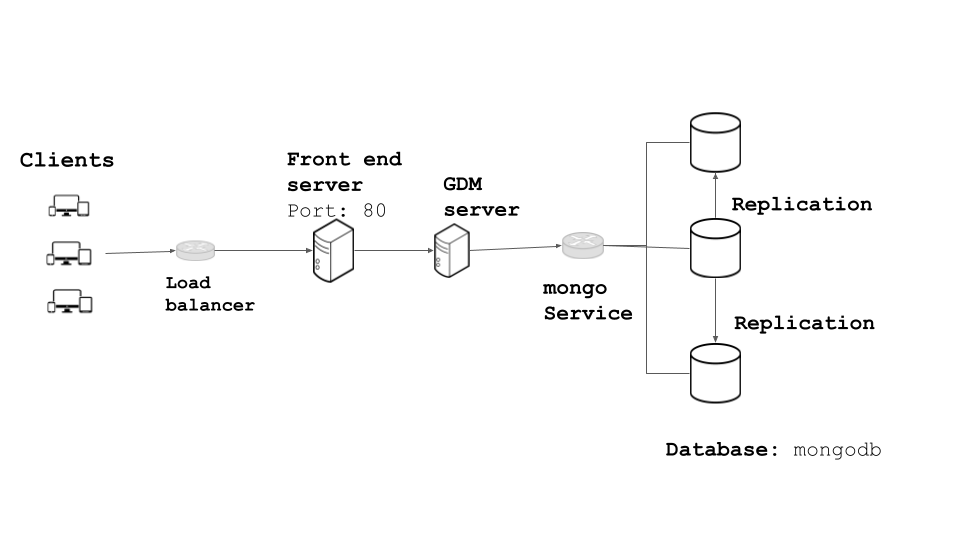
\includegraphics[width=1.0\linewidth]{project_slide.png}
    \caption{Architecture}
    \label{fig:enter-label}
\end{figure}

\subsubsection{Front End server}
The front end server is the entry point for clients. It exposes port 80 as the service endpoint and we've attached an external load balancer so that remote clients can communicated with the server. Front End server manages client sessions and implements the external API by aggregate responses from different rpcs made to the gdm server. The FE server queries GDM server for user data and also fetches the real time diagnosis based on latest patient metrics.

\subsubsection{GDM server}
The GDM server is the main microservice. It implements the GDM service below: 

\begin{lstlisting}
service Gdm {
    rpc GetSamples()
    rpc WriteSample()
    rpc SignUp()
    rpc SignIn()
    rpc GetUser()
    rpc GetDiagnosis()
}
\end{lstlisting}

The GDM server is also responsible for predicting whether a patient is at risk of GDM. It serves the pickled classifier and exposes the prediction as the GetDiagnosis rpc. The service runs on port 50051.

\subsubsection{Mongo DB }
MongoDB is our database of choice. We run a highly available mongo db service in our cluster. The service hosts 3 replicas and leader election is used to decide which replica to read / write to.

\subsubsection{Client simulator}
The client simulator is implemented as multiple clients signing up and periodically generating OGTT readings. We are able to run as many client replicas as we want to simulate. The simulator is a long lived service and continuously generates samples until it is killed.


\subsection{User End Web page - Doctor and Patient}
The web page's seamless integration of user input and glucometer data enables effective risk analysis and monitoring. It enables medical personnel to spot high-risk instances, personalise treatment regimens, and give pregnant GDM patients prompt interventions. This strategy promotes accurate risk assessment and focused management of GDM throughout the course of pregnancy by taking into account age, BMI, OGTT results, and ethnicity.

An essential part of the system is the User End Web page, which has patient and doctor dashboards. Its main goal is to promote excellent communication and seamless contact between pregnant patients and medical providers, enabling successful gestational diabetes (GDM) monitoring and management. This section will go into more detail about the functionality and design of the doctor and patient dashboards, which are built using MongoDB as the backend and HTML and CSS as the frontend.
\subsubsection{Doctor's Dashbaord}
Medical professionals, especially doctors and healthcare providers, can effectively manage and monitor their pregnant patients with Gestational Diabetes Mellitus (GDM) using the Doctor Dashboard, which is a comprehensive and user-friendly interface. With the use of this dashboard, doctors are better equipped to provide individualised and targeted care throughout the duration of pregnancy.
\begin{figure}[!htbp]
  \centering
  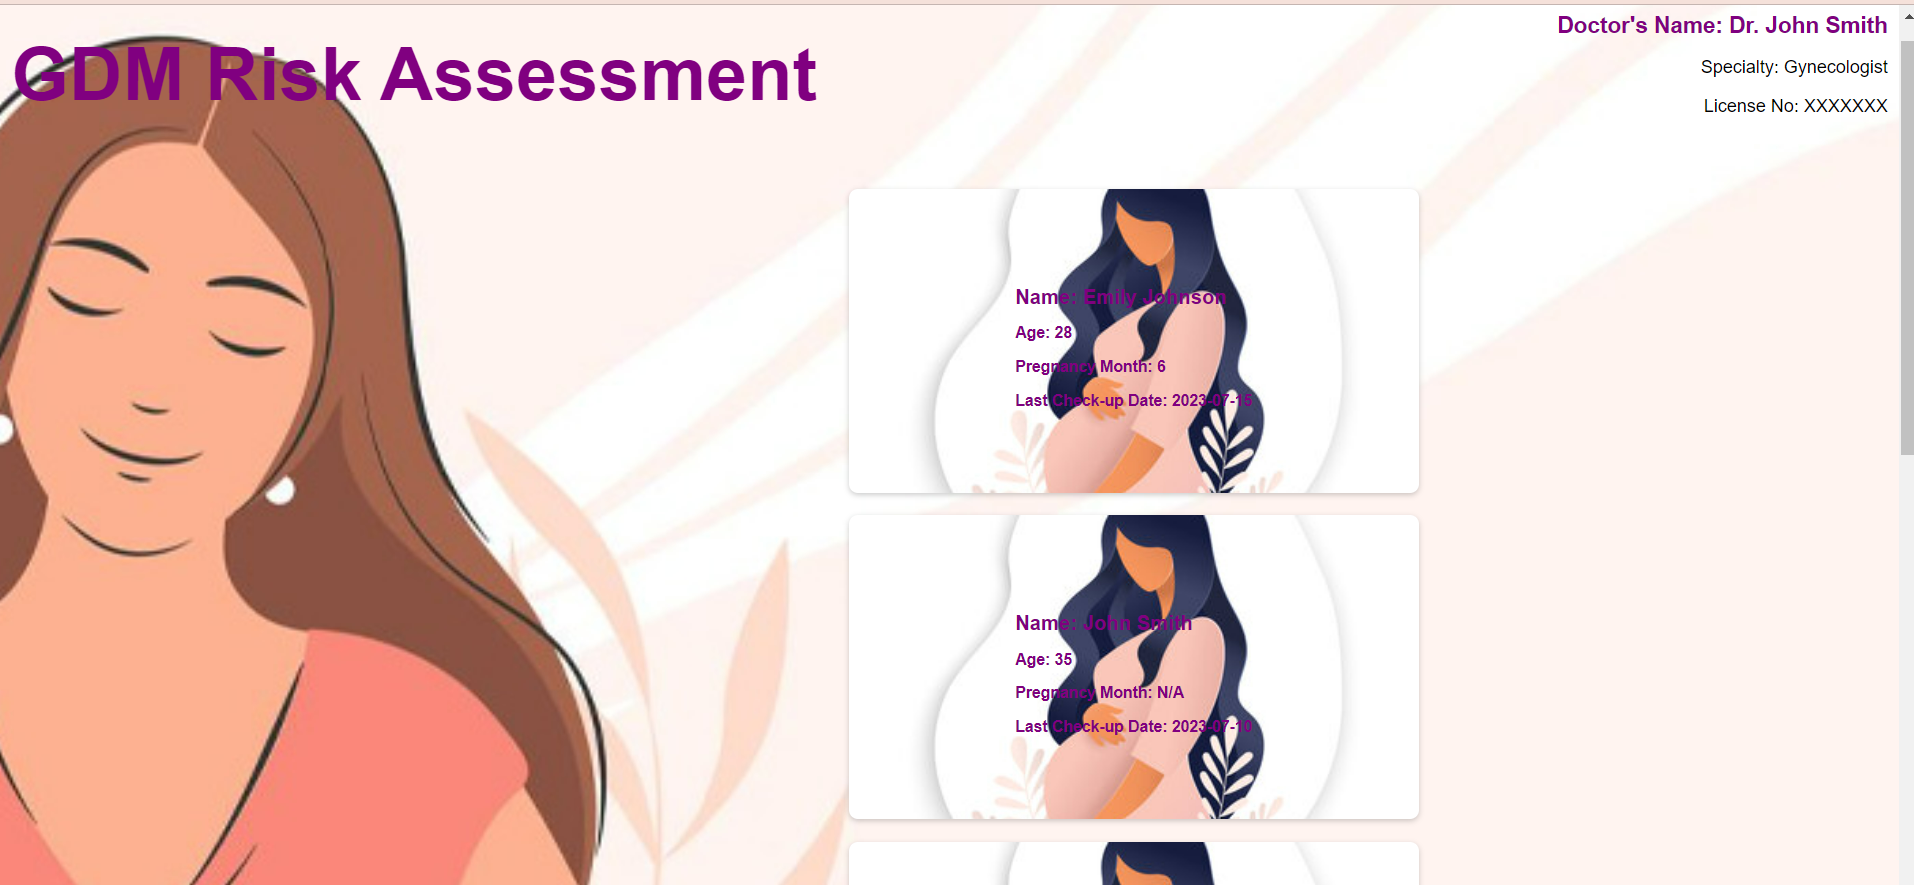
\includegraphics[width=0.8\columnwidth]{doc.png} % Replace with the actual path and filename of your image
  \caption{Doctors's Dashboard with all their Patients }
  \label{fig:glucometer_diag}
\end{figure}
\begin{figure}[!htbp]
  \centering
  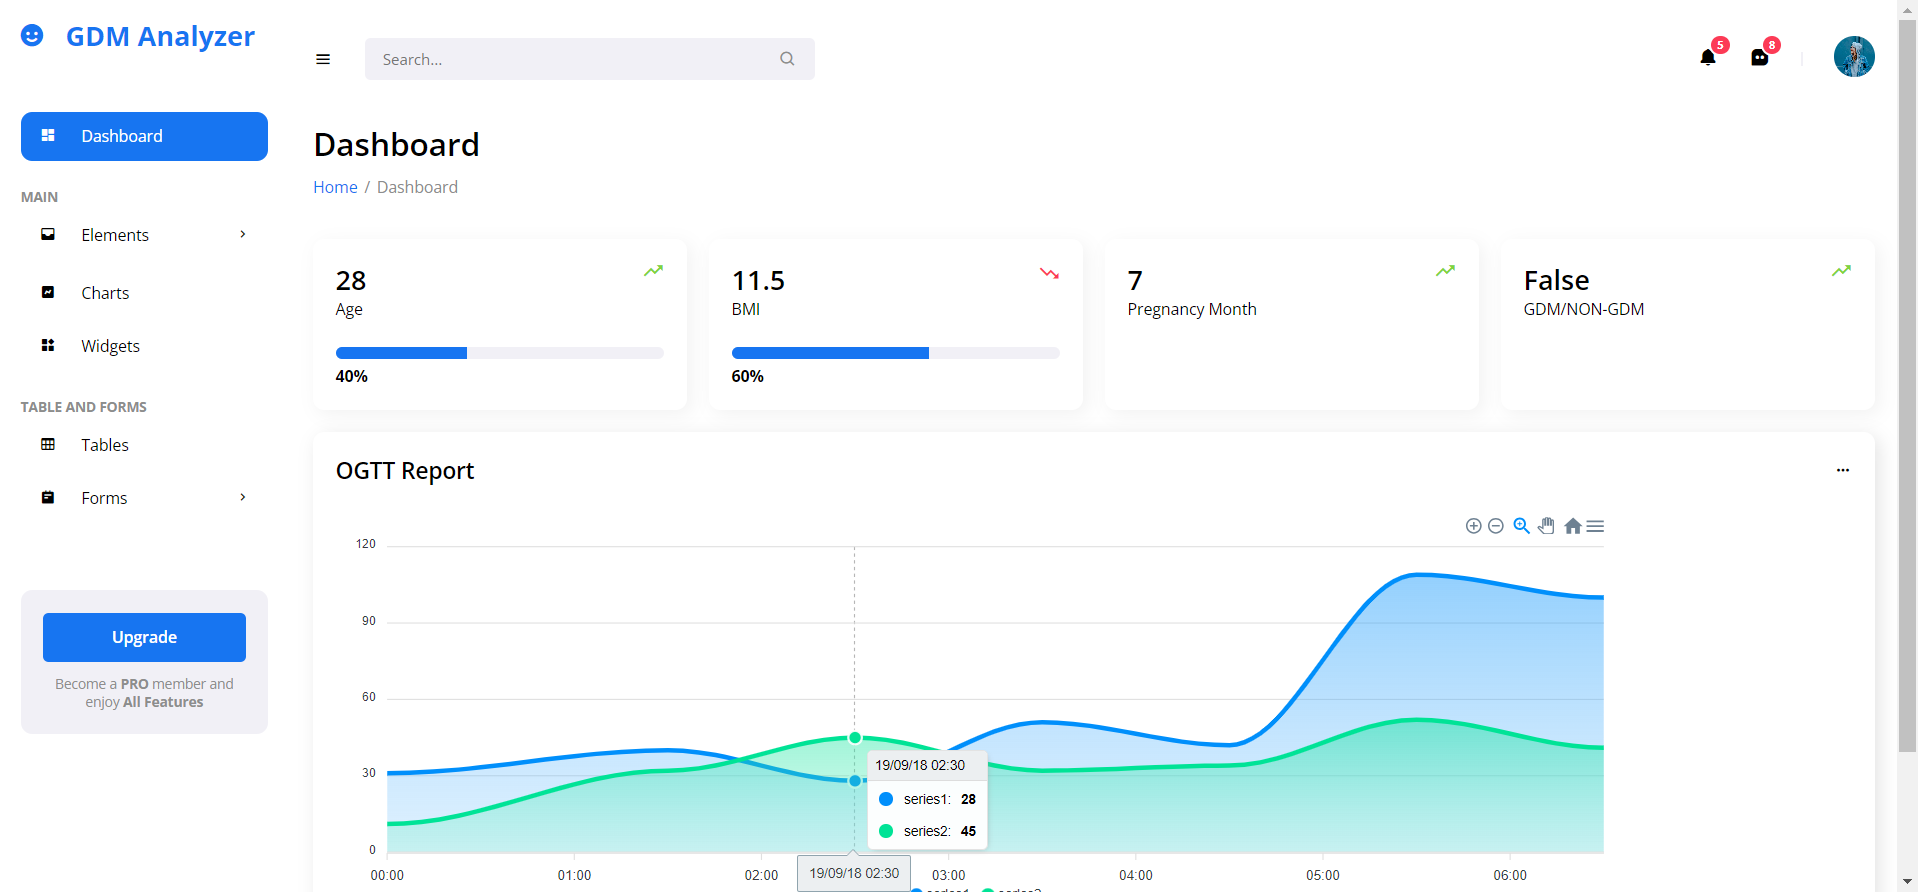
\includegraphics[width=0.8\columnwidth]{doc2.png} % Replace with the actual path and filename of your image
  \caption{Patient's Risk Analysis Dashboard from Doc's view}
  \label{fig:glucometer_diag}
\end{figure}
Key characteristics of the doctor's dashboard are as follows:
\begin{itemize}
    \item Patient Overview: All pregnant patients with GDM who are receiving care from the doctor are listed in a concise and organised manner on the doctor's dashboard. The display of vital patient data, such as name, age, gestational week, and contact information, enables doctors to retrieve each patient's record rapidly.
    \item Risk Analysis and Monitoring: To efficiently execute risk analysis for each patient, the dashboard combines user input and glucometer data. The system can identify high-risk situations and probable complications by taking into account variables like age, BMI, the results of the Oral Glucose Tolerance Test (OGTT), and ethnicity. This enables prompt interventions and customised treatment plans.
 \item Customizable Treatment Plans: The Doctor Dashboard enables medical staff to design individualised treatment plans for each patient based on the risk assessment and specific patient data. A patient's specific needs can be catered for when a doctor sets specific target glucose levels, suggests dietary changes, and prescribes proper drugs.
  \item Tools for Communication: The dashboard has outstanding communication options that enable easy communication between doctors and their patients. Regarding visits, medication schedules, and lifestyle advice, medical staff can send patients notifications, reminders, and critical updates.
\item Data Visualisation and Analytics: The dashboard makes use of data visualisation techniques to support precise risk assessment and targeted management. It is simpler for clinicians to spot patterns and modify treatment regimens when using graphs and charts to depict trends in patients' glucose levels over time.
\item Patient Progress Tracking: Using the doctor dashboard, doctors can keep tabs on how their pregnant patients are doing. They can view previous glucose data, assess the success of therapies, and base judgements on current information.
\item Simple Data Entry: The dashboard offers a user-friendly interface that makes it simple for doctors to enter and update patient data. It lessens the need for manual data entry, allowing medical staff to concentrate more on patient care.
\item Collaborative Care: The Doctor Dashboard can be connected with other healthcare systems in some installations, enabling collaborative care between the various healthcare professionals involved in the patient's treatment.
\end{itemize}
The Doctor Dashboard will be a crucial tool for healthcare providers to properly manage GDM patients, ensuring that they receive individualised care, ongoing monitoring, and prompt interventions. The dashboard equips doctors to make wise decisions, enhance patient outcomes, and deliver the greatest calibre of care throughout the critical stage of pregnancy with gestational diabetes mellitus by utilising technology and data analysis.

\subsubsection{Patient's Dashbaord}
The patient's parameters such as age,BMI, previous history of diabetes etc, which determines the diagnosis of GDM are acquired from the user's login/sign up page. This information is then sent to the GCP DBMS cloud to the predictive analysis model.
\begin{figure}[!htbp]
  \centering
  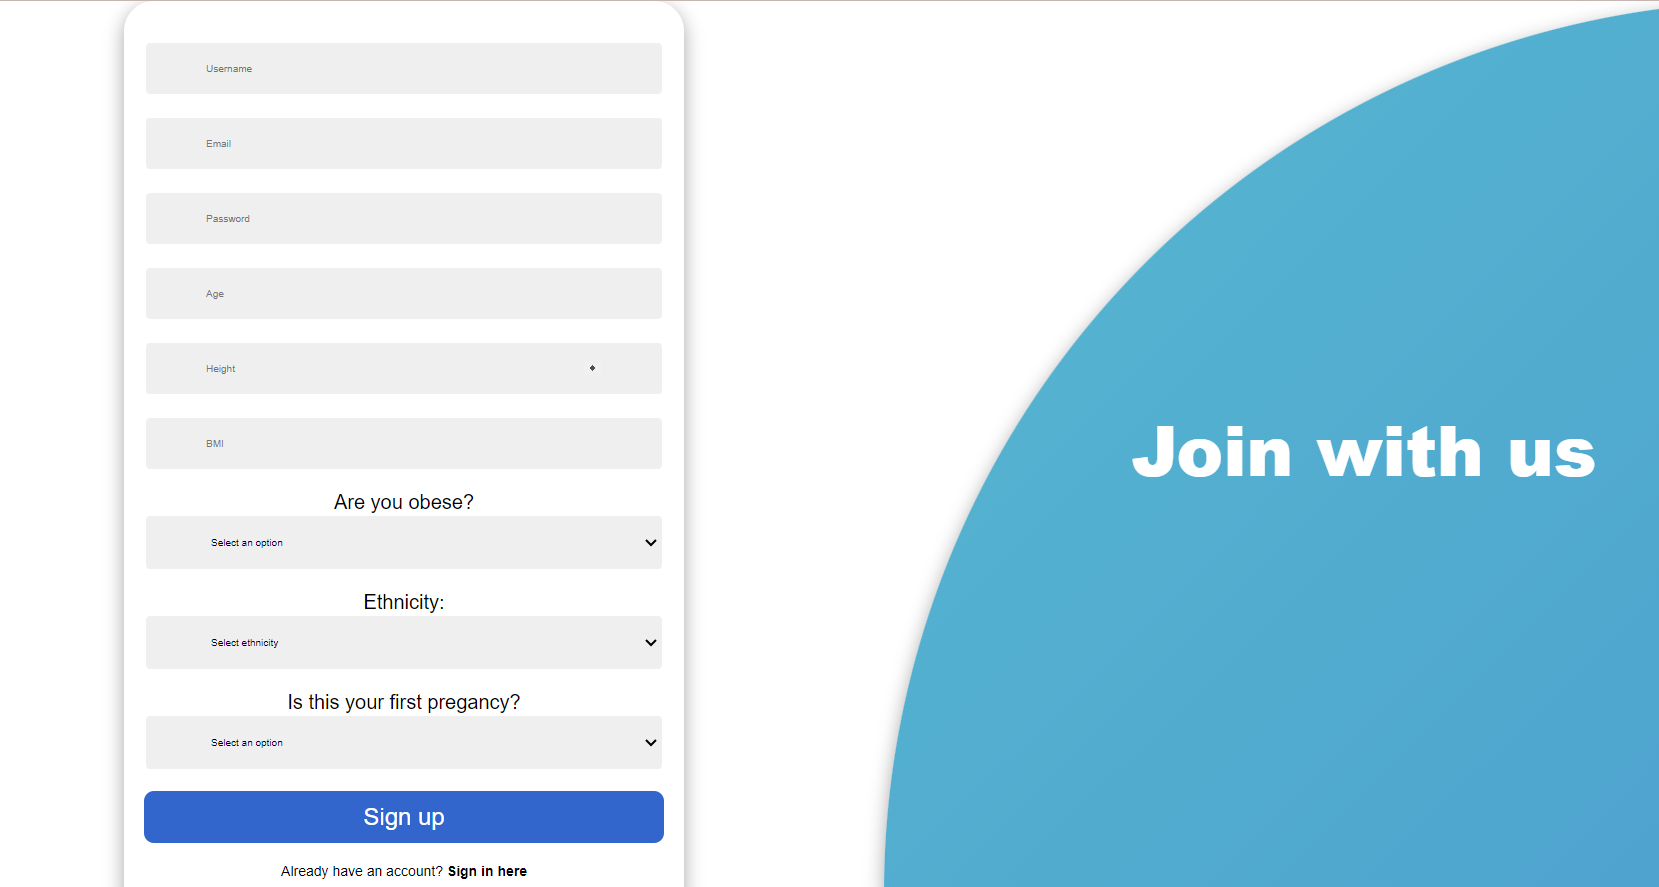
\includegraphics[width=0.8\columnwidth]{signup.png} % Replace with the actual path and filename of your image
  \caption{Patient's Sign up page }
  \label{fig:glucometer_diag}
\end{figure}
\begin{figure}[!htbp]
  \centering
  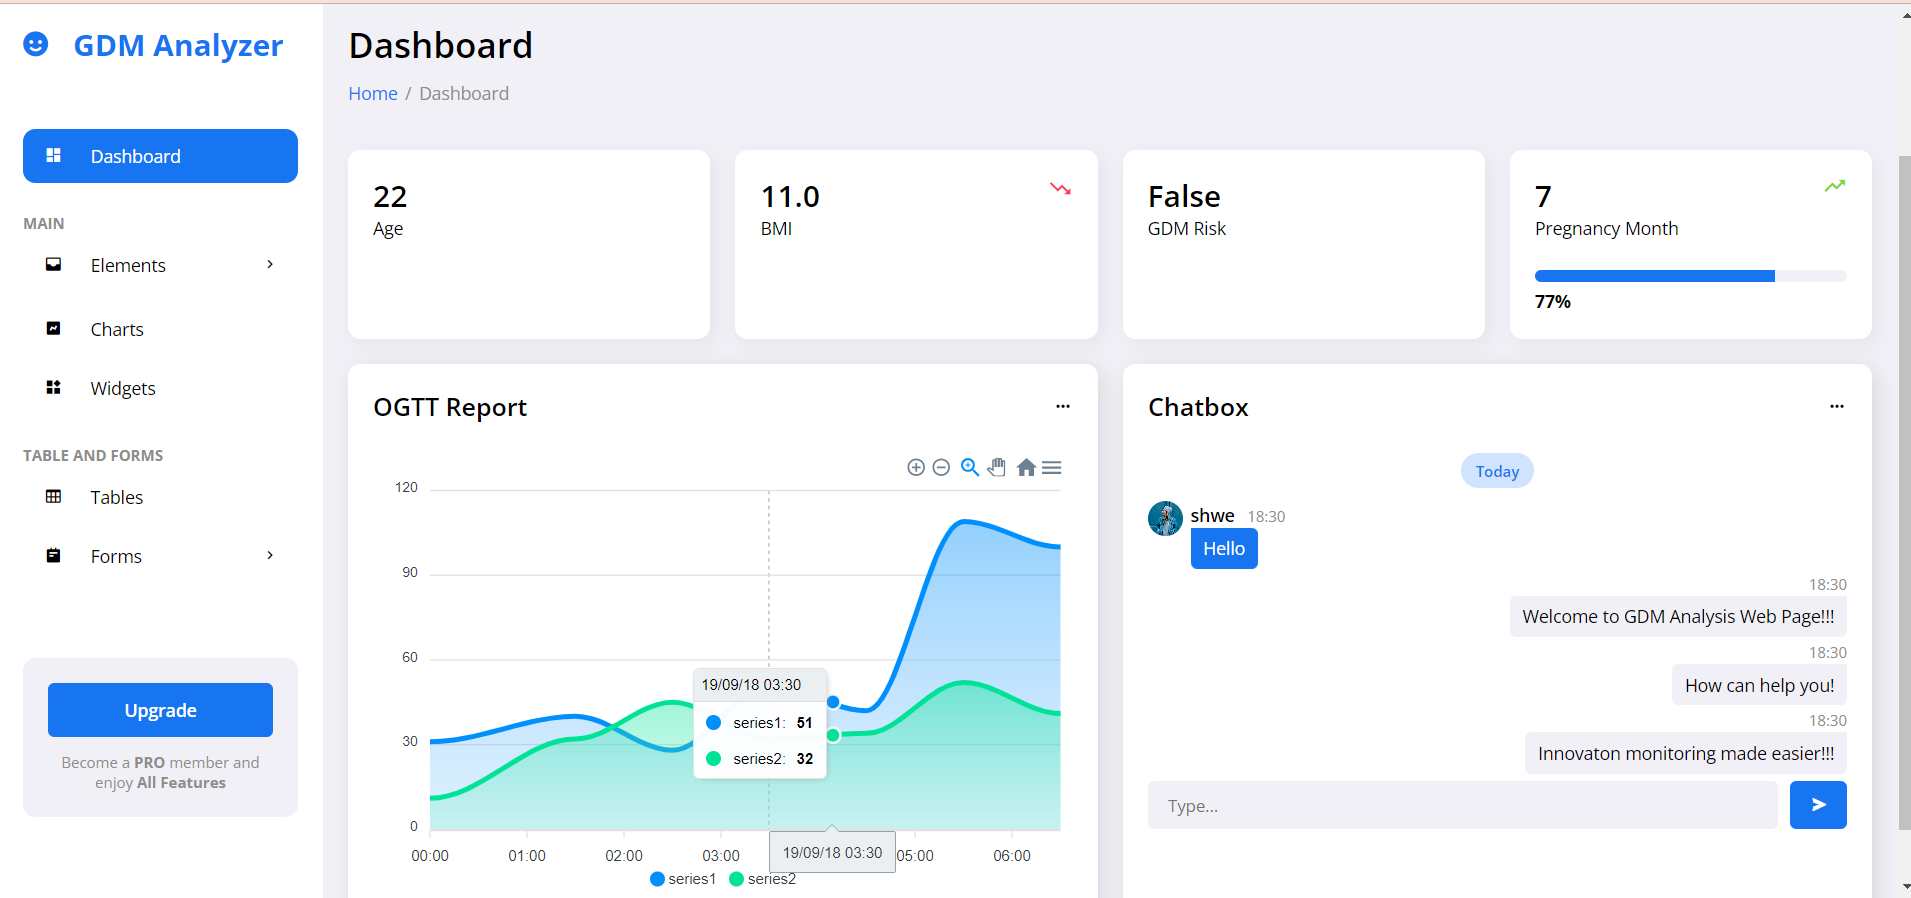
\includegraphics[width=0.8\columnwidth]{dash.png} % Replace with the actual path and filename of your image
  \caption{Patient's Risk Analysis Dashboard }
  \label{fig:glucometer_diag}
\end{figure}

The patient dashboard's functionality is designed to encourage pregnant women with GDM to take an active role in their healthcare. It provides the following crucial features:
\begin{itemize}
 \item Personalised Data Input: Through simple input forms, expectant patients can submit pertinent data including blood pressure, BMI, and glucose levels. Their health status may be continuously monitored thanks to this real-time data entry.
\item Visualisation of Glucose Trends: The patient dashboard shows glucose level trends over time using charts and graphs, allowing patients to understand the development of their condition graphically.
\item The dashboard includes a reminder and notification tool to encourage patients to regularly check their blood sugar levels and follow their treatment recommendations.
\item Patient Management: Access to patient profiles and medical histories enables thorough patient management and customised care regimens.

\item Risk Assessment and Decision Support: Using patient data, integrated ML/DL algorithms can help doctors assess the risks related to GDM, supporting well-informed clinical decision-making.

\item Access restrictions and encryption make sure that patient information stays private and is only available to licenced healthcare providers.

\item Communication and Follow-Up: Using the dashboard, medical professionals may have direct conversations with patients and provide them feedback, therapy modifications, and follow-up instructions.
\end{itemize}

\section{Conclusion and Future Scope}
Implementing this extensive action plan gives healthcare workers a strong toolkit to efficiently monitor glucose levels, evaluate risks, and proactively address the difficulties pregnant women with gestational diabetes (GDM) encounter. The initiative intends to allow coordinated treatment and improve the health of both the mother and the unborn child throughout the course of pregnancy by integrating cutting-edge technologies and encouraging seamless communication among pregnant women, healthcare professionals, and stakeholders.

The suggested approach involves real-time monitoring of expectant women using biosensors to gather crucial data like blood pressure, glucose levels, and BMI. However, due to ethical issues and practical limitations, gathering real-time data directly from pregnant women may cause difficulties. The project offers mimicking sensor data to get around this restriction. The study can still offer insightful information and help healthcare practitioners make decisions based on a thorough understanding of GDM by using simulated data.

The study also makes use of trained algorithms from public datasets to evaluate the dangers related to GDM. These models analyze the patient's vitals and forecast the likelihood and severity of problems including macrosomia and hypoglycemia using machine learning and deep learning techniques. The initiative can get beyond the drawbacks of real-time data collection while yet providing precise risk evaluations to aid clinical decision-making.

The project's essential component is effective communication between expectant mothers, healthcare professionals, and stakeholders. Applications for users and providers are created to make this connection easier. Healthcare practitioners may successfully monitor GDM, evaluate risks, and proactively address difficulties presented by expecting mothers by putting this thorough action plan into practice. The project's emphasis on effective stakeholder communication improves care coordination and makes sure that each patient's particular needs are satisfied. While collecting real-time data may be difficult, using trained models from internet datasets and simulated sensor data improves the project's viability. In the end, this strategy seeks to enhance maternal and fetal health, lessen problems, and foster better outcomes throughout the course of pregnancy.

The user web page can securely communicate with their healthcare providers through an integrated messaging system, ensuring timely information exchange and personalized advice.The dashboard may also include educational resources, providing patients with valuable information about GDM management, lifestyle changes, and self-care practices.

% conference papers do not normally have an appendix



% use section* for acknowledgment
\ifCLASSOPTIONcompsoc
  % The Computer Society usually uses the plural form
  \section*{Acknowledgments}
\else
  % regular IEEE prefers the singular form
  \section*{Acknowledgment}
\fi


The authors would like to extend their sincere appreciation and gratitude to Dr. Reena Prabha Kokila, Gynecologist from India, for her invaluable assistance, guidance, and expertise throughout the course of this research project. Dr. Kokila's profound insights, meticulous attention to detail, and unwavering support have been instrumental in shaping the success and quality of this work


% trigger a \newpage just before the given reference
% number - used to balance the columns on the last page
% adjust value as needed - may need to be readjusted if
% the document is modified later
%\IEEEtriggeratref{8}
% The "triggered" command can be changed if desired:
%\IEEEtriggercmd{\enlargethispage{-5in}}

% references section

% can use a bibliography generated by BibTeX as a .bbl file
% BibTeX documentation can be easily obtained at:
% http://mirror.ctan.org/biblio/bibtex/contrib/doc/
% The IEEEtran BibTeX style support page is at:
% http://www.michaelshell.org/tex/ieeetran/bibtex/
%\bibliographystyle{IEEEtran}
% argument is your BibTeX string definitions and bibliography database(s)
%\bibliography{IEEEabrv,../bib/paper}
%
% <OR> manually copy in the resultant .bbl file
% set second argument of \begin to the number of references
% (used to reserve space for the reference number labels box)
\begin{thebibliography}{1}

\bibitem{Saha2014}
S. Saha, N. Sarker, and A. Hira, "Design  Implementation of a Low Cost Blood Glucose Meter with High Accuracy," in \emph{International Conference on Electrical Engineering and Information \& Communication Technology (ICEEICT) 2014}, pp.
\bibitem{Kurt2023}
    B. Kurt, B. Gürlek, S. Keskin, et al., "Prediction of gestational diabetes using deep learning and Bayesian optimization and traditional machine learning techniques," \emph{Med. Biol. Eng. Comput.}, 2023. [Online]. Available: \url{https://doi.org/10.1007/s11517-023-02800-7}.

    \bibitem{ElRashidy2022}
    N. El-Rashidy, N.E. ElSayed, A. El-Ghamry, et al., "Prediction of gestational diabetes based on explainable deep learning and fog computing," \emph{Soft Comput}, vol. 26, pp. 11435-11450, 2022. [Online]. Available: \url{https://doi.org/10.1007/s00500-022-07420-1}.


    \bibitem{Dataset}
    Srirangan Jeyaparam, "GDM Dataset Figshare," [Online]. Available: \url{https://figshare.com/articles/dataset/GDM_Dataset_xlsx/21806472}
    
\end{thebibliography}


% that's all folks
\end{document}


